\subsection{Discrete Regularized Transport} 
\label{sec:regsymme}

So far, we have introduced a transport problem where the mass conservation constraint is relaxed. The second step is to define its regularization. A classic way of imposing regularity on a mapping $V: \RR^d \rightarrow \RR^d$ is by measuring the amplitude of its derivatives. Two examples for continuous functions are the quadratic Tikhonov regularizations such as the Sobolev semi-norm $\|\nabla V\|^2$, and the anisotropic total variation semi-norm $\|\nabla V\|_1$ regularization. But, the differential operator $\nabla$  cannot be applied directly to our point clouds due to the lack of neighborhood definition. To extend the definition of the gradient operator, we need to impose a graph structure on each point cloud.

In our setting, we want to regularize the discrete map $T$ defined in~\eqref{eqT}, which is only defined at the location of the points as $X_i \mapsto \tilde{V}_i=X_i - \diag(\Sig \U)^{-1} (\Sig Y)_i $.  To avoid the normalization $\diag(\Sig \U)$ (which typically leads to non-convex optimization problems) we impose a regularity on the map $X_i \mapsto V_i = \diag(\Sig \U)X_i-(\Sigma Y)_i$. This switch also has the advantage of imposing a stronger regularization in regions with large weights and to further regularize the variations of the weights $\Sig \U \in \RR^N$. We believe these are actually interesting features to reduce artifacts for imaging applications. 

\paragraph{Gradient on Graphs}

A natural way to define a gradient on a point cloud $X$ is by using  the gradient on a weighted graph $\Gg_X = (X,E_X,W_X)$ where $E_X \subset \{1,\ldots,N\}^2$ is the set of edges and $W_X$ is the set of weights, $W_X = (w_{i,j})_{i,j=1}^N:  \{1,\ldots,N\}^2 \mapsto \RR^+$, satisfying $w_{i,j}=0$ if $(i,j) \notin E_X$. The edges of this graph are defined depending on the application. A typical example is the $n$-nearest neighbor graph, where every vertex $X_i$ is connected to $X_j$ if $X_j$ is one of the $n$-closest points to $X_i$ in $X$, creating the edge $(i,j) \in E_X$, with a weight $w_{i,j}$. Because the edges are directed, the adjacency matrix is not symmetric. 

The gradient operator on $\Gg_X$ is defined as $G_X : \RR^{N \times d} \rightarrow \RR^{P \times d}$, where $P=\|E_X\|$ is the number of edges and where, for each $V=(V_i)_{i=1}^N \in \RR^d$, 
\eq{
	G_X V = \pa{ w_{i,j}(V_i-V_j) }_{(i,j) \in E_X} \in \RR^{P \times d}.
}
A classic choice for the weights to ensure consistency with the directional derivative is $w_{i,j} = \norm{X_i-X_j}^{-1}$, see for instance~\cite{guilboa07}.


%%%%%%%%%%%%%%%
\paragraph{Regularity Term}

The regularity of a transport map $V \in \RR^{N \times d}$ is then measured according to some norm of $G_X V$, that we choose here for simplicity to be the following
\eq{
	\regul{G_X  V} = \sum_{(i,j) \in E_x} \left(\norm{ w_{i,j} (V_i-V_j) }_q \right)^p,
}
where $\|.\|_q$ is the $\ell^q$ norm in $R^d$. 

The case $(p,q)=(1,1)$ is the graph anisotropic total variation, $(p,q)=(2,2)$ is the graph Sobolev semi-norm, and $(p,q)=(1,2)$ is the graph isotropic total variation, see for instance~\cite{elmoataz-graph} for applications of these functionals to imaging problems such as image segmentation and regularization. 

\subsection{Symmetric Regular OT Formulation}

Given two point clouds X and Y, our goal is to compute a relaxed OT mapping between them which is regular with respect to both point clouds. To simplify notation, we conveniently re-write the displacement fields we aim to regularize as:
\eq{
	\De_{X,Y}(\Sig) = \diag( \Sigma \U ) X - \Sigma Y
	\qandq
	\De_{Y,X}(\Sig^*) = \diag( \Sigma^* \U ) Y -  \Sigma^* X.
}

Our goal is to obtain a partial matching that is regular according to $X$ and $Y$, so we create two graphs $\Gg_X$ and $\Gg_Y$ as described in Section~\ref{sec:regsymme} and we denote the corresponding gradient operators $G_X \in \RR^{P_X \times N}$ and $G_Y \in \RR^{P_Y \times N}$ where $P_X$ and $P_Y$ are the number of edges in the respective graphs. The symmetric regularized discrete OT energy is defined as: 
\eql{\label{eq-symm-reg-energy}
\umin{\Sig \in \Matr_\kappa} \dotp{\Sig}{\Cost{X}{Y}} + \la_X \regul{G_X \De_{X,Y}(\Sig)} + \la_Y \regul{G_Y \De_{Y,X}(\Sig^*)},
}
where $(\la_X,\la_Y) \in (\RR^+)^2$ controls the desired amount of regularity.
The case $\kappa=(1,1,1,1)$ and $(\la_X,\la_Y)=(0,0)$ corresponds to the usual OT defined in~\eqref{eqMK}, and $(\la_X,\la_Y)=(0,0)$ corresponds to the un-regularized formulation~\eqref{eq-relax-map}.

%%%%%%%%%%%%%%%
\subsection{Algorithms} 
\label{secalgosymm}

Specific values of the parameters $p$ and $q$ lead to different regularization terms, which in turn necessitate different optimization methods. In the following, for the sake of concreteness, we concentrate on the specific cases $(p,q)=(2,2)$ and $(p,q)=(1,1)$.

%%%
\paragraph{Sobolev regularization}

Defining $q=p=2$ fixes the regularization term as a graph-based Sobolev regularization. In this specific case, the minimization~\eqref{eq-symm-reg-energy} becomes a quadratic programming problem 
\begin{equation} \label{eq-symm-S}
	\umin{\Sig \in \Matr_\kappa}
	f(\Sig) =  \dotp{ \Cost{X}{Y}}{\Sig } + \frac{\la_X}{2} \norm{ \Gamma_{X,Y}(\Sig)\|^2 + \frac{\la_Y}{2} \|\Gamma_{Y,X}(\Sig) }^2, 
\end{equation} 
where $\Gamma_{X,Y}(\Sig) = G_X \De_{X,Y}(\Sig)$ and $\Gamma_{Y,X}(\Sig) = G_Y \De_{Y,X}(\Sig^*)$. The Frank-Wolfe algorithm is well tailored to solve such problems, as noticed for instance in~\cite{Zaslavskiy09}, given that $f$ is convex and differentiable, and $\Matr_\kappa$ is a convex set. 
The Frank-Wolfe method (also known as conditional gradient) iterates the following steps until convergence
\begin{equation}
\begin{aligned}\label{eq-frankwolfe-update}
	\tilde\Sig^{(\ell+1)} &\in \uargmin{\tilde\Sig \in \Matr_\kappa} \dotp{\nabla f(\Sig^{(\ell)})}{ \tilde\Sig } \\
	\Sig^{(\ell+1)} &= \Sig^{(\ell+1)} + \tau_\ell ( \tilde\Sig^{(\ell+1)}-\Sig^{(\ell+1)} ),\\
\end{aligned}
\end{equation}
where $\tau_\ell$ is obtained by line-search. The first equation of~\eqref{eq-frankwolfe-update} is a linear program which is efficiently solved using interior point methods~\cite{Nesterov-Nemirovsky-Book}. 
The function $f$ is quadratic, and to compute $\nabla f(\Sig)$, we note that $\nabla \frac{1}{2}\norm{\Ga_{X,Y}(\Sig)}^2 = \Ga_{X,Y}^*( \Ga_{X,Y}(\Sig) )$, where the adjoint $\Ga_{X,Y}^*$ of $\Ga_{X,Y}$ is
\eq{
	\Ga_{X,Y}^* = \De^*_{X,Y} \circ G_X^*
	\qwhereq 
	\choice{
		\De^*_{X,Y}(U)= \diag^*(U X^*)\U^*-U Y^*, \\
		\De^*_{Y,X}(U)= (\diag^*(U Y^*)\U^*)^*-X U^*,
	}
}
where $\diag^*: \RR^{N \times N} \mapsto \RR^{N}$ is the adjoint of the $\diag$ operator, and given $A \in \RR^{N \times N}$, $\diag^*(A)$ is a vector composed by the elements on the diagonal of $A$. 

This leads to the following formula
\eq{
	\nabla f(\Sig) = \Cost{X}{Y} + \la_X  \De^*_{X,Y}(G_X^*  \Gamma_{X,Y}(\Sig)) + \la_Y \De^*_{Y,X}(G_Y^* \Gamma_{Y,X}(\Sig)), 
} 

The line search optimal step can be explicitly computed as
\eq{
	\tau_{\ell} = 
	\frac{ - \dotp{ E^{(\ell)} }{ 
		\Cost{X}{Y} } - 
		\dotp{  \Gamma_{X,Y}(E^{(\ell)}) }{  \Gamma_{X,Y}(\Sig^{(\ell)}) } - 
		\dotp{  \Gamma_{Y,X}( E^{(\ell)} )  }{  \Gamma_{Y,X} (\Sig^{(\ell)}) }	
	}{ 
		\la_X \norm{\Gamma_{X,Y}(E^{(\ell)})}^2 +   \la_Y \norm{\Gamma_{Y,X}(E^{(\ell)})}^2
	}
} 
where $E^{(\ell)} = \Sig^{(\ell+1)} - \tilde\Sig^{(\ell+1)}$.

%%%%
\paragraph{Anisotropic TV regularization}

We define an anisotropic total variation (TV) norm by setting the parameters $q=p=1$.
Problem~\eqref{eq-symm-reg-energy} can be re-written as a linear program by introducing the auxiliary variables $U_X \in \RR^{P_X \times d}$ and $U_Y \in \RR^{P_Y \times d}$
\eql{
\begin{aligned}
& \underset{\Sig, U_X,U_Y}{\text{min}}  & & \dotp{ \Cost{X}{Y}}{\Sig}  + \lambda_X \dotp{U_X}{\U}+ \lambda_Y \dotp{U_Y}{ \U} \\
& \mbox{subject to} & &
\left\{ \begin{aligned}
-U_X  & \leq G_X ( \Sig Y  - \diag(\Sig \U) X)\leq U_X, \\
-U_Y & \leq G_Y( \Sig^* X - \diag(\Sig^* \U) Y) \leq U_Y, \\
\Sig & \in \Matr_\kappa. \\
\end{aligned}
\right.
\end{aligned}\label{eq-symm-TV}
}

%%%%
\paragraph{Numerical illustrations}

In Fig.~\ref{exlk}, we can observe, on a synthetic example, the influence of the parameters $\kappa$ and $(\lambda_X, \lambda_Y)$, from equation~\eqref{eq-symm-reg-energy}. 

\begin{figure*}\label{figlambda}
\centering
\begin{tabular}{@{}|@{}c@{}|@{}c@{}|@{}}
\hline
  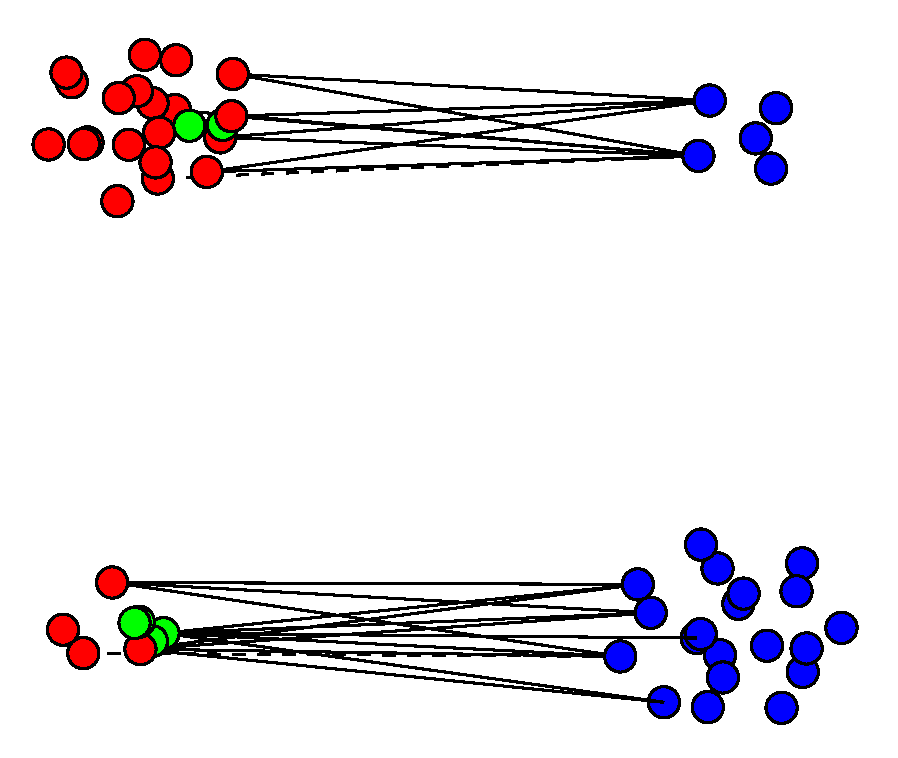
\includegraphics[width=.4\linewidth]{../images/syntheticexamples/symmetricsyntheticmapping_l0_KX8_KY8_nn4} &  
  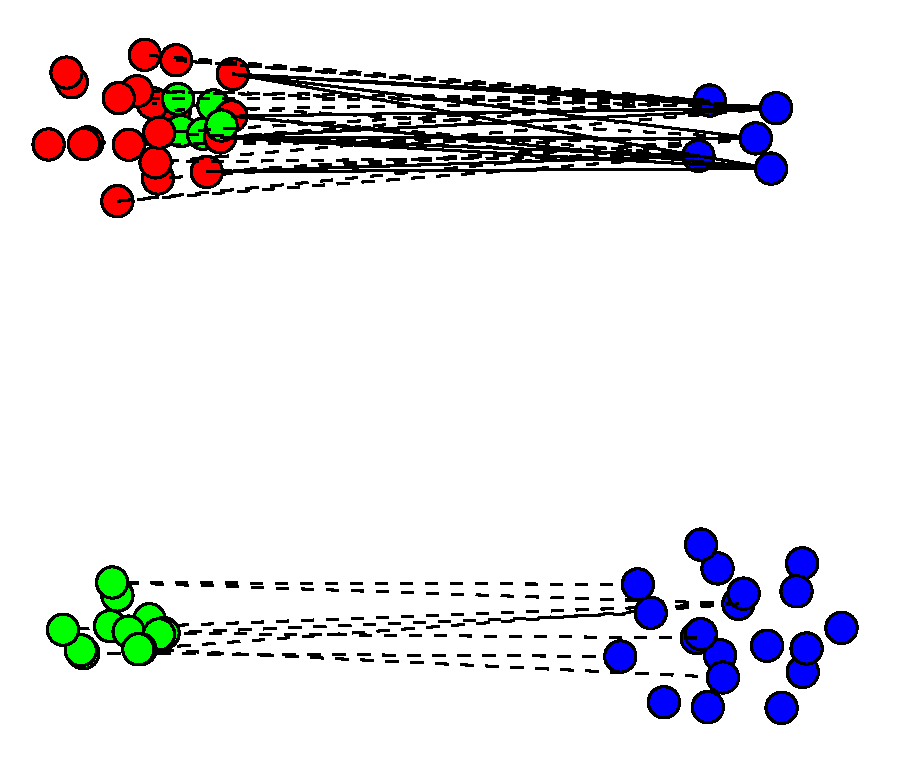
\includegraphics[width=.4\linewidth]{../images/syntheticexamples/symmetricsyntheticmapping_l0001_KX8_KY8_nn4} \\
	 {$\la_X=\la_Y=0$} & {$\la_X =\la_Y=0.001$}\\\hline
  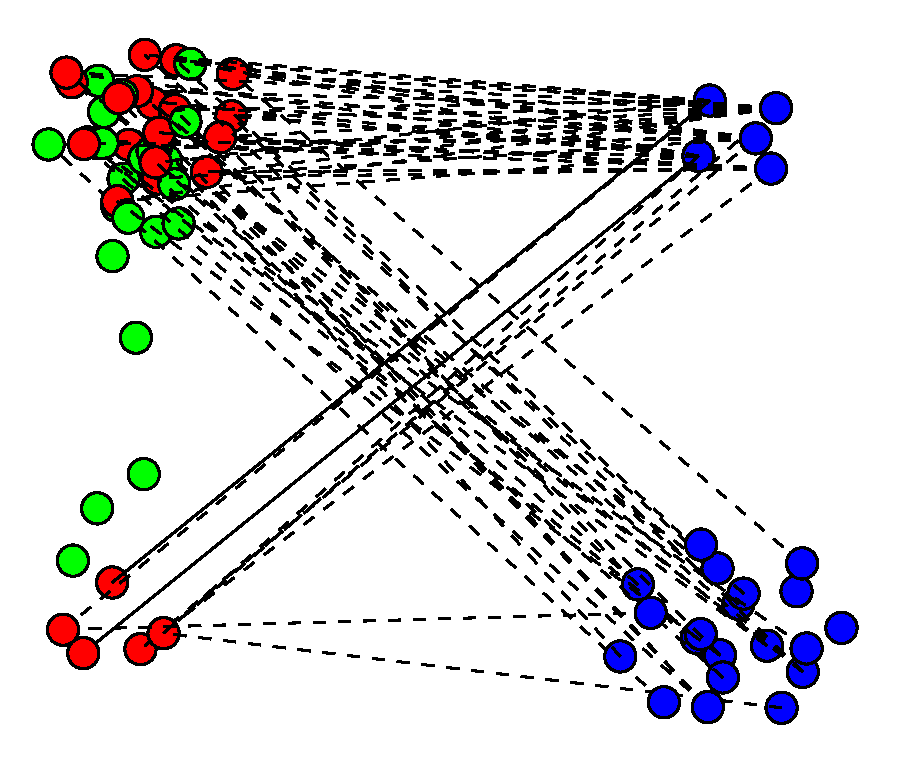
\includegraphics[width=.4\linewidth]{../images/syntheticexamples/symmetricsyntheticmapping_l10_KX8_KY8_nn4} &
  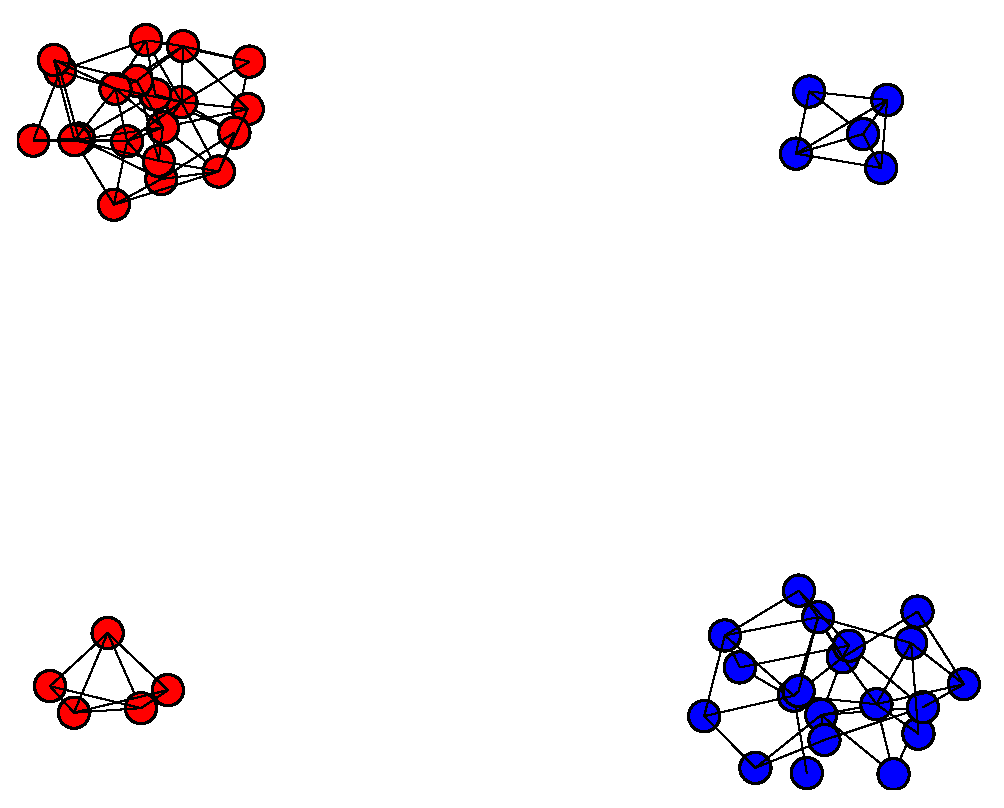
\includegraphics[width=.4\linewidth]{../images/graph} \\  
  {$\la_X =\la_Y=10$} & Graphs \\\hline 
\end{tabular}
\caption{Given two sets of points $X$ (in blue) and $Y$ (in red), we show the points $Z=\diag(\Sigma \U)^{-1} \Sigma Y$ (in green), and the mappings $\Sigma_{i,j}$ as line segments connecting $X_i$ and $Y_j$, which are dashed if $\Sigma_{i,j} \in ]0.1,1[$  and solid if $\Sigma_{i,j}=1$. The results were obtained with the relaxed and regularized OT formulation, setting the parameters to $\kappa=(0.1,8,0.1,8)$. Note the influence of a change in $\la_X$ and $\la_Y$ on the final result: with no regularization ($\la_X=\la_Y=0$) only few points in the data set are matched. The introduction of regularization ($\la_X=\la_Y=0.001$) spreads the connections among the clusters, while maintaining the cluster-to-cluster matching. For  a high value of $\la_X=\la_Y=10$, the regularization tends to match the clusters with similar shape with each other, where the shape is defined by the graph structure. The graphs $\Gg_X$ and $\Gg_Y$ are represented with the nodes on blue and red respectively, and the edges as solid lines.}\label{exlk}
\end{figure*}

For $\la_X=\la_Y=0$ one obtains the relaxed symmetric OT solution, where the transport maps the points in $X$ to the closest point on $Y$, and vice versa. As we increase the values of $\la_X$ and $\la_Y$ to $0.001$, we can see how the regularization affects the mapping. Let us analyze $\regul{G_X \De_{X,Y}(\Sig)} = \|G_X \diag(\Sig \U) X - G_X \Sig Y\|^2 $, for instance. The  term $G_X \diag(\Sig \U) X$ is measuring the regularity of the weights $\diag(\Sig \U)$ on $X$ and the consequence is that for $\la_X=\la_Y=0.001$ there are 
plenty of connections with low weight (there are few solid lines), while for $\la_X=\la_Y=0$ there are several mappings with $\Sig_{i,j} = 1$ (solid lines). So, the regularization promotes a spreading of the matchings. 

The minimum of $\regul{G_X \De_{X,Y}(\Sig)}$ is reached when $G_X \diag(\Sig \U) X = G_X \Sig Y$, that is, when the graph structure of $X$ has the same shape as the graph structure of $\Sig Y$, which both can be observed in the last column and row. For high values of $\la_X=\la_Y$ the matchings tend to link the clusters by their shape, that is, the big cluster on $X$ with the big cluster of $Y$, and similarly for the small clusters (note that the links with higher value are between the small clusters). 


